\section{Application on cardiac electrophysiology simulation}

Simulations of cardiac electrophysiology have become a valuable tool for the
study and comprehension of the heart's bioelectric activity under normal and
pathological conditions. These simulations are usually based on the bidomain
model~\cite{Sundnes2006Book}, which is a system of two partial differential
equations (PDEs) coupled to a set of nonlinear ordinary differential equations
(ODEs) describing the behavior of the membrane of cardiac cells. In spite of
being currently the most complete description of the electrical activity of the
heart, the numerical solution of the bidomain equations is a computational
challenging task~\cite{Weber2004}. Usually the bidomain equations are reduced to
the simpler monodomain model by considering that: the extracellular potential is
constant; or tissue conductivity is isotropic; or the intracellular and
extracellular conductivities have equal anisotropy
ratios~\cite{Sundnes2006Book}.

\subsection{Monodomain Model}

In cardiac tissue, the excitation wave spreads through the tissue because
the cardiac cells are electrically coupled via special proteins called
gap junctions. This phenomenon is mathematically described by a
reaction--diffusion equation referred to as the monodomain equation, given by
\begin{align}
   \beta C_m \DP{V_m}{t} + \beta I_{ion}(V_m,\bs{\eta}) &=
   \nabla \cdot (\bs{\sigma_m} \nabla V_m) + I_{stim}\\
\DP{\bs{\eta}}{t} &= \bs{f}(V_m, \bs{\eta})
   \label{eq:Monodomain}
\end{align}
where $\beta$ is the surface-to-volume ratio of the cardiac cells,
$C_m$ is the membrane capacitance, $V_m$ is the transmembrane voltage,
$I_{ion}$ is the density of the total ionic current which is a function of
$V_m$ and a vector of state variables $\bs{\eta}$, $I_{stim}$ is a stimulus
current and $\bs{\sigma_m}$ is the monodomain conductivity tensor. The tissue
is assumed to be isolated along its boundaries, i.e. no--flux boundary
conditions are imposed on $V_m$ along all myocardial surfaces.

In this work the classical Luo--Rudy I (LRI) model~\cite{Luo1991} that describes the
electrical activity in a general mammalian ventricular cell was considered to
simulate the kinetics of $I_{ion}$ in Eq.~\eqref{eq:Monodomain}. In this
mammalian ventricular model, $I_{ion}$ is defined as the following sum of
currents:
\begin{equation}
   I_{ion} = I_{Na} + I_{si} + I_{K} + I_{K1} + I_{Kp} + I_{b}
   \label{eq:LRDI}
\end{equation}
where $I_{Na}$ is the fast sodium current, $I_{si}$ is the slow inward current,
$I_{K}$ is the time-dependent potassium current, $I_{K1}$ is the
time-independent potassium current, $I_{Kp}$ is the plateau potassium current
and $I_{b}$ is time-independent background current. The LRI model is based on a
set of 8 ODEs describing ionic currents and intracellular calcium concentration.
For a full specification of the model and its ionic currents see~\cite{Luo1991}.

\subsection{Finite Volume model applied to monodomain}

In this section we will make a brief description of the Finite Volume Method (FVM) applied to the
monodomain equations. Details about the FVM applied to monodomain can be found
in~\cite{harrild1997finite} and ~\cite{coudiere20092d}.

The reaction and diffusion part of the monodomain equations can be split by
employing the Godunov operator splitting~\cite{Sundnes2006Book}. Each time step involves the solution of two different problems: a nonlinear system of ODEs
\begin{align}
  \DP{V_m}{t} &= \frac{1}{C_m} \left[ - I_{ion} (V_m,\eta_i) + I_{stim} \right]
  \label{eq:Step1a} \\
  \DP{\eta_i}{t} &= f(V_m, \eta_i) \label{eq:Step1b}
\end{align}
 and a parabolic linear PDE
\begin{align}
  \DP{V_m}{t} &= \frac{1}{\beta C_m}
  \displaystyle\left[ \nabla \cdot (\bs{\sigma} \nabla V_m) \right]
  \label{eq:Step2}
 \end{align}

Depending on the numerical method, the spatial discretization
of the parabolic PDE results in a linear system of equations
that have to be solved at each time step.

\subsubsection{Time discretization}

The time derivative present in Equation~\eqref{eq:Step2}, which operates on $V$
is approximated by an implicit first--order Euler scheme:
\begin{equation}
\frac{\partial V}{\partial t} = \frac{V^{n+1}-V^{n}}{\Delta t},
\label{eq:tempo}
\end{equation}
where $V^{n}$ represents the transmembrane potential at time
$t_{n} $ and $\Delta t$ the increment at every step.

\subsubsection{Space discretization}

The diffusion term of Equation~\eqref{eq:Step2} needs to be spatially
discretized. To do this we will consider the following relations:
\begin{equation}
  J = -\sigma \nabla V
  \label{eq:ji}
\end{equation}
where $J$ $(\mu A/cm^2)$ represents the density of the intracellular current
flow and
\begin{equation}
  \nabla \cdot J = -I_v.
  \label{eq:iv}
\end{equation}

In this expression, $I_v (\mu A/cm^3)$ is a volumetric current and corresponds
the left side of Equation~\eqref{eq:Step2}.

For simplicity, we will consider a tri-dimensional uniform mesh, consisting  of
cubes (called ``Volume''). Situated in the center of each volume
is a node and $V$ is associated with each node of the mesh.

After defining the geometry of the mesh and the partitioning of the domain
in control volumes, the FMV-specific equations can be presented.
The Equation ~\eqref{eq:iv} can be integrated spatially over a cube
specific, leading to:

\begin{equation}
  \int_{\Omega} \nabla \cdot J da = -\int_{\Omega} I_v \, da.
\end{equation}
applying the divergence theorem, we find that
\begin{equation}
  \int_{\Omega} \nabla \cdot J da = \int_{\partial \Omega} J \cdot \vec{\eta},
\end{equation}
where $\vec{\eta}$ is the vector normal to the edge.

Finally, assuming that $ I_v$ represents an average value in each particular
cube, and substituting in Eq~\eqref{eq:Step2}, we have the following
relationship:
\begin{equation}
    \beta\left (C_m \dfrac{\partial V}{\partial t} \right)\bigg|_{(i,j,k)}
     = \dfrac{-\int_{\partial \Omega} J \cdot \vec{\eta}}{h^3},
     \label{eq:mono2}
\end{equation}
where $h^3 $ is the volume of the control cell and $\vec{\eta}$
represents the vector normal to the surface.

For the three-dimensional problem, formed by a uniform grid of cubes with
face area $h^2$, the calculation of $J$ can be split as the sum of the flows
on the six faces:
\begin{equation}
          \int_{\partial \Omega} J \cdot \vec{\eta} = h^2 \cdot \displaystyle
          \sum_{l=1}^{6}{{Jf}_l}
     \label{eq:flux}
\end{equation}
where,
\begin{eqnarray}
  \sum_{l=1}^{6}{{Jf}_l} &=& J_{x_{i+1/2,j,k}} - J_{x_{i-1/2,j,k}} \nonumber \\
                      &+& J_{y_{i,j+1/2,k}} - J_{y_{i,j-1/2,k}} \\
                      &+& J_{z_{i,j, k+1/2}} - J_{z_{i,j, k-1/2}} \nonumber,
\end{eqnarray}

The tensor $\sigma = \left(\begin{array}{ccc} \sigma_x & 0 & 0 \\ 0 & \sigma_y &
0 \\ 0 & 0 & \sigma_z \end{array} \right)$ must be determined at the interfaces
of the volume. For this, we use the harmonic mean:
\begin{eqnarray}
    \sigma_{x_{i+1/2, j}} = \displaystyle \dfrac{2\sigma_{x_{i,j}}\sigma_{x_{i+1,j}}}{\sigma_{x_{i+1, j}}+\sigma_{x_{i,j}}}
     % \sigma_{x_{i-1/2, j}} = \displaystyle \dfrac{2\sigma_{x_{i,j}}\sigma_{x_{i-1,j}}}{\sigma_{x_{i-1, j}}+\sigma_{x_{i,j}}}.
\end{eqnarray}

A similar reasoning can be used to calculate $\sigma_{x_{i-1/2, j,
k}}$, $\sigma_{y_{i, j+1/2, k}}$, $\sigma_{y_{i, j-1/2}}$, $\sigma_{z_{i, j,
k+1/2}}$ and $\sigma_{z_{i, j, k-1/2}}$.

The flows $J_{x_{m,n,o}}$, $J_{y_{m,n,o}}$ and $J_{y_{m,n,o}}$ are calculated in the
faces ($(m,n,o)$ = $(i+1/2,j,k)$, $(i-1/2,j,k)$, $(i,j+1/2,k)$, $(i,j-1/2,k)$,
$(i,j,k+1/2)$ or $(i,j,k-1/2)$) as follows:

\begin{eqnarray}
    J_{x_{m,n,o}} = \sigma_x(m,n,o) \dfrac{\partial V}{\partial x} \bigg|_{(m,n,o)}\\
    J_{y_{m,n,o}} = \sigma_{y}(m,n,o) \dfrac{\partial V}{\partial y} \bigg|_{(m,n,o)}\\
    J_{z_{m,n,o}} = \sigma_{z}(m,n,o) \dfrac{\partial V}{\partial z} \bigg|_{(m,n,o)}
\end{eqnarray}

\subsubsection{Adaptive non-uniform mesh (ALG)}

In this section we present the application of the FVM using an adaptive non-
uniform mesh, in this case ALG. For this, we will approximate the partial derivatives of $V$ on
the interfaces using the following finite difference scheme, considering uniform
discretizations in space ($\Delta x = \Delta y = \Delta z = h$):
\begin{eqnarray}
    \label{eq:dvdx1}
    \dfrac{\partial V}{\partial x} \bigg|_{(i+1/2,j,k)} = \dfrac{V_{i+1,j,k} - V_{i,j,k}}{h}
\end{eqnarray}
The equations for $y$ and $z$ can be obtained similarly.

Rearranging and replacing the discretizations of the equations~\eqref{eq:tempo}
and~\eqref{eq:flux} in Equation~\eqref{eq:mono2} and decomposing the
operators as described by the equations~\eqref{eq:Step1a}, \eqref{eq:Step1b} and~
\eqref{eq:Step2} we have:
\begin{eqnarray}
C_m \dfrac{V^{*}_{i,j,k} - V^{n}_{i,j,k}}{\Delta t} &=&\dfrac{h^2 \cdot \displaystyle
          \sum_{l=1}^{6}{{Jf^*}_l} }{\beta h^3} \\
C_m \dfrac{V^{n+1}_{i,j,k} - V^{*}_{i,j,k}}{\Delta t} &=& -I_{ion}(V^*_{i,j,k},\bs{\eta}^n) \\
\dfrac{\partial \bs{\eta}^{n+1}}{\partial t} &=& f(\bs{\eta}^n, V^*, t)
\end{eqnarray}
where:
\begin{eqnarray}
%%%%%%J_{i+1/2,j}%%%%%%%%%%
   J^*_{x_{i+1/2,j}} =
   \sigma_{x_{i+1/2,j,k}} \dfrac{V^{*}_{i+1,j,k} - V^{*}_{i,j,k}}{h},
   \label{eq:fluxo1}
\end{eqnarray}
Eq.~\eqref{eq:fluxo1} represents the flow of the cell (i, j, k) by the right
face of the cube to the neighbor cell, $n$ is the current step, $*$ is
an intermediate step and $n+1$ is the next time step. Equations for
$J^*_{x_{i-1/2,j,k}}$, $J^*_{y_{i,j+1/2,k}}$, $J^*_{y_{i,j-1/2,k}}$,
$J^*_{z_{i,j, k+1/2}}$ and $J^*_{z_{i,j, k-1/2}}$ can be obtained similarly.
Developing all equations, we can now define the time advance formula for
the interior points of each volume:
\begin{align}
\label{eq:sis_so}
\nonumber
(\sigma_{x_{i+1/2,j,k}}+\sigma_{x_{i-1/2,j,k}} +\sigma_{y_{i,j+1/2,k}} + \sigma_{y_{i,j-1/2,k}} \sigma_{x_{i,j,k+1/2}}+\sigma_{x_{i,j,k-1/2}} + \alpha) V^*_{i,j,k} + \\ \nonumber
\sigma_{y_{i,j-1/2,k}} V^*_{i,j-1,k} -\\ \nonumber
\sigma_{x_{i+1/2,j,k}} V^*_{i+1,j,k} -\\ \nonumber
\sigma_{z_{i,j,k+1/2}} V^*_{i,j,k+1} -\\ \nonumber
\sigma_{y_{i,j+1/2,k}} V^*_{i,j+1,k} -\\ \nonumber
\sigma_{x_{i-1/2,j,k}} V^*_{i-1,j,k}  =
V^t_{i,j,k}*\alpha,
\end{align}
where $\alpha = (\beta C_m h^2)/\Delta t$.

Algorithm \ref{mono_alg} describes the steps used for the numerical resolution
of monodomain model. As can be seen, we have to reassemble the monodomain
matrix at each time step if a refinement or derefinement operation has been
performed in that step. In this example application, the criteria used for
refinement and derefinement are based on the flux across the interface of
neighboring cells. That is, if the absolute value of the flux is larger than a
predefined refinement threshold ($reft$), the program chooses to refine this
cell, whereas if the absolute value of the flux of all four cells of a bunch is
less than an derefinement threshold ($dreft$), the program chooses to derefine
the bunch. For the monodomain application, the values for the refinement and
derefinement thresholds where empirically found.
\alglanguage{pseudocode}
\begin{algorithm}[!ht]
    \caption{Steps used for the numerical resolution of monodomain model}
    \small{
    \begin{algorithmic}[1]
        \State set cell model initial conditions;
        \State assemble the monodomain matrix (Linear system form PDE);
        \While{$t < final\_t$}
        \State update cell Model state vector;
        \State solve cell model;
       \State solve linear system (PDE) via conjugate gradient method;
        \State refine-derefine
       \State reassemble the monodomain matrix if needed;
       \State $t = t + dt$
        \EndWhile
    \end{algorithmic}
    }
    \label{mono_alg}
\end{algorithm}

Figure~\ref{SIM_ALG3D} shows the simulation results using ALG adaptive mesh. We can
clearly see that the region delimited by the wavefront has a spatial discretization
smaller than the rest of the tissue. The colors represents the distribution of
transmembrane potential V.

\begin{figure}
    \centering
    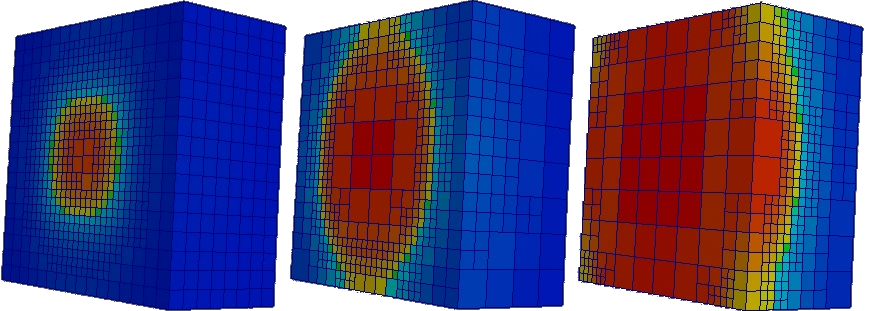
\includegraphics[scale=0.40]{../img/onda3d.png}
    \caption{Simulation using ALG adaptivity scheme. Result of the simulated
electric wave propagation (distribution of transmembrane potential V ) in a ventricular
tissue.}
    \label{SIM_ALG3D}
\end{figure}
